%% AASTeX v7 manuscript, typeset two-column.  Every display fits a single
%% column; drop [twocolumn] for the one-column manuscript layout, or add
%% [linenumbers] for review.
\documentclass[twocolumn]{aastex701}

\usepackage{amsmath}
\usepackage{bm}
\usepackage{array}
\newcolumntype{L}[1]{>{\raggedright\arraybackslash}p{#1}}
\usepackage{tikz}
\usetikzlibrary{positioning,arrows.meta,fit,calc,backgrounds}

\newcommand{\vect}[1]{\bm{#1}}
\newcommand{\dd}{\mathrm{d}}
\newcommand{\yes}{$\checkmark$}

\shorttitle{LVM sky subtraction}
\shortauthors{Drory}

\begin{document}

\title{Sky Subtraction for the Local Volume Mapper:\\
Physical Decomposition and Learned Sky-to-Science Transfer}

\author{Niv Drory}
\affiliation{The University of Texas at Austin, Austin, TX, USA}
\email{droryn@eid.utexas.edu}

\begin{abstract}
We describe a sky-subtraction procedure for the SDSS-V Local Volume Mapper
(LVM) in which the sky spectrum at the science pointing is predicted from two
simultaneous sky pointings. Each of the three spectra of an exposure is first
decomposed into physically distinct emitters --- OH and O$_2$ airglow, atomic
lines, the diffuse airglow continuum, scattered moonlight and zodiacal light
--- by a constrained quadratic program. The program fits the instrumental
line-spread function and the telluric attenuation of the airglow jointly with
the amplitudes, and it uses hard linear constraints to make the
moonlight/zodiacal-light and diffuse-continuum partitions identifiable. The
resulting coefficient vectors are normalised for line-of-sight geometry and
extinction in closed form, and a neural network with physically motivated
coefficient groups, isolated branches for the anisotropic emitters and an
explicit arm-blend prior predicts the science-pointing coefficients from the
two sky pointings and the observing context. Amplitudes that the
decomposition fixes by constraint rather than by data are derived from
geometry at prediction time instead of being learned. The predicted
coefficients are reconstructed into a full-resolution sky spectrum and
subtracted from the science exposure.
\end{abstract}

%% Replace with Unified Astronomy Thesaurus concepts and their IDs.
\keywords{Night sky brightness --- Airglow --- Zodiacal light ---
Astronomy data reduction --- Neural networks}

%======================================================================
\section{Problem statement}
\label{sec:problem}

LVM \citep{Drory2024} observes extended, low-surface-brightness emission from
the Milky Way and the Magellanic Clouds, for which the night sky is a
first-order contaminant. Each science exposure is accompanied by two
simultaneous sky exposures taken with dedicated sky telescopes pointed at
blank fields a few degrees from the science field. The sky is not uniform on
this baseline:
\begin{itemize}
  \item scattered moonlight has strong angular structure set by the
        scattering phase functions of molecules and aerosols;
  \item the zodiacal light varies by tens of percent with ecliptic latitude
        and elongation across the pointings of one night;
  \item OH airglow is modulated by mesospheric gravity waves on scales of
        tens of arcminutes;
  \item the three lines of sight have different zenith angles and hence
        different slant paths through the emitting layers and the
        atmosphere.
\end{itemize}
Subtracting either sky spectrum directly therefore leaves systematic
residuals of order one to ten percent of the sky, enough to bury the diffuse
emission that motivates the survey.

The procedure described here replaces direct subtraction by a prediction.
Each spectrum is decomposed into per-emitter coefficients
(Section~\ref{sec:decomp}). The coefficients are transformed to a
geometry-normalised, zenith-equivalent frame (Section~\ref{sec:geometry}). A
learned transfer (Section~\ref{sec:ml}) maps the two sky pointings and the
observing context to the coefficients at the science pointing at the same
instant. The predicted coefficients are reconstructed into a sky spectrum on
the native pixel grid and subtracted from the science spectrum.

%======================================================================
\section{Input data}
\label{sec:inputs}

\paragraph{Instrument.} The LVM instrument comprises separate telescopes for
science, for two sky fields (east and west) and for spectrophotometric
standards, all feeding fibre bundles into spectrographs with three channels
($b$, $r$, $z$) covering $3600$--$9800$\,\AA. The fibre diameter is
$35.3''$. The two sky telescopes point at fields chosen near the science
field; for each exposure we call the one that is closer on the sky the
\emph{near} arm and the other the \emph{far} arm. This assignment varies from
exposure to exposure and is independent of which physical telescope is used.

\paragraph{Spectra.} The inputs are the reduced, flux-calibrated frames of
the LVM data reduction pipeline (DRP). The DRP divides every fibre by a model
telluric transmission evaluated along the \emph{science} line of sight; this
matters for the decomposition (Section~\ref{sec:telluric}). For each exposure
we form three spectra on a common grid of $N_\lambda = 12\,401$ pixels at
$\Delta\lambda = 0.5$\,\AA:
\begin{itemize}
  \item the median over the science fibres, after rejecting fibres whose
        Gaia DR3 \citep{GaiaDR3} predicted stellar $G$-band flux exceeds
        1\% of the fibre's measured flux plus sky;
  \item the median over the fibres of each sky telescope.
\end{itemize}
The median is a robust estimate of the sky-dominated spectrum. Its variance
is that of a mean over $N_{\rm eff} = (2/\pi)\,n_{\rm fib}$ fibres, where
$n_{\rm fib}$ is the number of fibres combined. Each spectrum carries the
per-pixel line-spread function (LSF) width of its fibre bundle.

\paragraph{Metadata.} Each exposure provides:
\begin{itemize}
  \item the pointing coordinates of all three telescopes;
  \item the exposure mid-time and duration;
  \item the airmass of each pointing;
  \item the precipitable water vapour (PWV) used by the DRP;
  \item the identity of the near and far telescopes.
\end{itemize}
Solar, lunar and ecliptic geometry are computed from these for each pointing
(Section~\ref{sec:ctx}), together with solar and geomagnetic activity indices
for the date.

\paragraph{Sample.} The sample used here contains $18\,668$ exposures. A
\emph{row} is one exposure with its three spectra (science, near, far).
$13\,688$ rows survive the selection of Section~\ref{sec:selection}.

%======================================================================
\section{Physical decomposition}
\label{sec:decomp}

Each of the three spectra of a row is fitted independently by the same
physical model. The model returns a non-negative coefficient vector
$\vect{c}\in\mathbb{R}^{P}$ with $P = 388$, together with its uncertainty,
the component spectra and a set of reliability flags. The coefficients are
the quantity the transfer of Section~\ref{sec:ml} operates on. The
decomposition is therefore designed so that each coefficient has a fixed
physical identity from row to row, even where the data alone could not
enforce it.

\subsection{Model}
\label{sec:model}

The observed spectrum is written as a non-negative linear combination of
templates:
\begin{equation}
  y(\lambda) \;\simeq\; \sum_{k=1}^{P} c_k\,T_k(\lambda), \qquad c_k \ge 0 ,
  \label{eq:model}
\end{equation}
where each template $T_k$ is a physical spectrum convolved with the fitted
LSF of the row (Section~\ref{sec:lsf}), attenuated by the atmosphere as
appropriate for its emitting layer (Section~\ref{sec:telluric}), and divided
by the transmission the DRP removed. Stacking the templates gives the design
matrix
\begin{equation}
\begin{split}
  \mathbf{A} = \big[\,&\mathbf{A}_{\rm OH}\,\big|\,\mathbf{A}_{\rm O_2}\,\big|\,
  \mathbf{A}_{\rm atom}\,\big|\\
  &\mathbf{A}_{\rm moon}\,\big|\,\mathbf{A}_{\rm zodi}\,\big|\,
  \mathbf{A}_{\rm diff}\,\big]
  \in \mathbb{R}^{N_\lambda\times P}.
\end{split}
\end{equation}
The families are listed in Table~\ref{tab:families}. They divide into a
\emph{line} block (OH, O$_2$, atomic lines), which depends on the LSF, and a
\emph{continuum} block (moonlight, zodiacal light, diffuse airglow), which is
smooth on the scale of the LSF. This division structures the estimation
(Section~\ref{sec:estimation}).

\begin{deluxetable}{lrL{11.2cm}}
\tablecaption{Emitter families of the decomposition.\label{tab:families}}
\tablehead{\colhead{Family} & \colhead{$n$} & \colhead{Template}}
\startdata
OH Meinel bands & 357 & groups of PALACE transitions sharing the upper
  vibrational level $v'$, rotational level $N'$ and fine-structure component
  $F'$; ridge-corrected relative line strengths \\
O$_2$ atmospheric ($b$) band & 1 & per-row band shape from a pre-fit \\
Atomic lines & 7 & K\,\textsc{i} 7699, Na\,\textsc{i}\,D, [O\,\textsc{i}] 5577;
  N\,\textsc{i} 5199, [O\,\textsc{i}] 6300/6364, O\,\textsc{i} 7774,
  O\,\textsc{i} 8446 \\
Scattered moonlight & 15 & solar spectrum $\times$ lunar albedo $\times$ cubic
  B-spline multiplier (11 interior knots) \\
Zodiacal light & 5 & reddened solar spectrum $\times$ cubic B-spline
  multiplier (1 interior knot) \\
Diffuse airglow continuum & 3 & HO$_2$, FeO and O$_2$ continuum templates \\
\hline
Total & 388 & \\
\enddata
\end{deluxetable}

\subsection{Line-spread function}
\label{sec:lsf}

Every narrow template depends on the LSF, which varies with wavelength and
between spectrograph channels. We represent the LSF kernel at wavelength
$\lambda$ as a continuous probability density in the offset
$\delta = \lambda' - \lambda$:
\begin{equation}
  K(\delta;\lambda) = \sum_{j=1}^{11} a_j(\lambda)\,M_j(\delta),
  \qquad \sum_j a_j(\lambda) = 1 .
  \label{eq:lsf}
\end{equation}
Here the $M_j$ are cubic M-splines on equally spaced knots over
$|\delta|\le3$\,\AA, each normalised
to unit integral, so $K$ integrates to one. The fit constrains the kernel to
be non-negative and unimodal, with a single central peak, at every
wavelength. The weights vary smoothly with wavelength within each channel: they are constant
in the $b$ channel and a six-function cubic B-spline in $\lambda$ in the $r$
and $z$ channels. A line template is rendered by integrating
$K(\,\cdot\,;\lambda_\ell)$ analytically over each pixel for every line
$\ell$ of the family. The LSF parameters are fitted to the sky lines of the
row itself (Section~\ref{sec:estimation}), with a roughness penalty on the
weights and a low-order polynomial nuisance background in each channel. A
Gaussian of the DRP-reported width seeds the fit, and it is retained for any
channel that carries too little line information to constrain the kernel. The same fitted LSF
convolves the continuum templates, where it has little effect.

\subsection{Atmospheric transmission}
\label{sec:telluric}

The airglow is emitted at 85--300\,km and reaches the telescope through the
whole lower atmosphere. The OH Meinel bands in the red and near-infrared
overlap the H$_2$O and O$_2$ absorption bands. If undimmed templates were
fitted, the line amplitudes would absorb the transmission. That transmission
depends on airmass and water vapour, so it would not cancel between the
pointings, and the transfer would be asked to predict atmospheric absorption
disguised as mesospheric emission. Two corrections avoid this:
\begin{enumerate}
  \item Each line template is attenuated at its own centre wavelength by the
        PALACE molecular transmission, evaluated from high-resolution line
        optical depths at the airmass $X_{\rm src}$ of the fibre being
        fitted:
        \begin{equation}
          t_\ell = \exp\!\Big\{-X_{\rm src}\big[\tau_\ell^{\rm dry}
          + (w/w_0)\,\tau_\ell^{\rm H_2O}\big]\Big\},
        \end{equation}
        where $w$ is the PWV and $w_0 = 2.5$\,mm is the reference water
        column.
  \item Every template is divided by the smooth transmission
        $T_{\rm DRP}(\lambda;\,X_{\rm sci},w)$ that the DRP removed from all
        fibres along the science line of sight. Model and data are then
        compared in the frame in which the data are delivered.
\end{enumerate}
The row's design matrix is therefore
$\mathbf{A}^{\rm row} = \mathbf{A}(X_{\rm src}, w)/T_{\rm DRP}(\lambda;
X_{\rm sci}, w)$, and the coefficients keep the meaning of
top-of-atmosphere amplitudes of the emitting layer. Compared with a fit that
omits the transmission, this lowers the decomposition $\chi^2$ by about 30\%
over the full band, with essentially no change in the blue, where there is no
telluric absorption. Integrated amplitudes
$A_g = \vect{c}_g\cdot\vect{v}_g$ are always defined with the
transmission-free template integrals $\vect{v}_g$, so they measure the
emission itself.

\subsection{OH and O$_2$ airglow}
\label{sec:oh}

OH nightglow dominates the sky beyond about 6000\,\AA, and the LVM
resolution separates individual rotational transitions. The model contains
357 OH templates. Each is the sum of the PALACE \citep{Noll2025} transitions
that share $(v', N', F')$, with relative strengths taken from a population
model. Grouping by upper state lets the fit follow changes in the rotational
and vibrational populations, which trace mesospheric temperature and
chemistry, while keeping the number of free parameters well below the number
of transitions.

\paragraph{Ridge-corrected line strengths.} The relative line strengths
within each group are a linear correction of the PALACE population model.
The correction was fitted on far-arm sky spectra with ridge regularisation
($\lambda_{\rm ridge} = 0.1$). The correction mainly repairs lines in the
$r$ channel. There the canonical relative strengths are too weak by about
0.11\,dex. The fit could not compensate, because those lines share
coefficients with the brighter $z$-channel lines of the same upper state. On
1000 test rows the correction:
\begin{itemize}
  \item reduces the decomposition $\chi^2$ on OH-dominated pixels by factors
        of 33 in $r$ and 3.6 in $z$, and by 31\% over the full band, with
        every row improving;
  \item reduces the systematic residual at the OH lines, stacked over rows,
        from 1.1\% to 0.14\% of the line peak in $r$;
  \item leaves the coefficients themselves nearly unchanged (0.8\% at the
        90th percentile), and leaves the continuum partition and all
        reliability flags unchanged.
\end{itemize}
Because the coefficients hardly change, any reconstruction must use the same
line strengths as the fit: a mismatch is invisible in coefficient space and
appears only in flux.

\paragraph{O$_2$ atmospheric band.} The O$_2$ $b$-band near 8645\,\AA{} is
first fitted on its own. The resulting per-row band shape then enters the
main fit as a single template with one free amplitude.

\subsection{Atomic lines}

Seven atomic features enter as single templates. The mesopause lines are
K\,\textsc{i} 7699, Na\,\textsc{i}\,D and [O\,\textsc{i}] 5577. The
thermospheric (F-region) lines are N\,\textsc{i} 5199,
[O\,\textsc{i}] 6300/6364 and the O\,\textsc{i} 7774 and 8446 recombination
lines. The distinction matters for the geometric normalisation
(Section~\ref{sec:heights}).

\subsection{Scattered moonlight}
\label{sec:moonfam}

Scattered moonlight is the dominant broadband contaminant with the Moon up.
Its template family is
\begin{equation}
  T_{{\rm moon},j}(\lambda) = I_\odot(\lambda)\;
  \alpha_{\rm ROLO}(\lambda,\phi_0)\; B^{(11)}_j(\lambda),
\end{equation}
for $j = 1,\dots,15$. The terms are:
\begin{itemize}
  \item $I_\odot$ is the solar spectrum \citep{Meftah2018};
  \item $\alpha_{\rm ROLO}$ is the disk-integrated lunar albedo
        \citep{Kieffer2005} at a fiducial phase angle
        $\phi_0 = 30^\circ$;
  \item $B^{(11)}_j$ are cubic B-splines with 11 interior knots across the
        band.
\end{itemize}
The spline multiplier absorbs the wavelength dependence of atmospheric
scattering and the departure of the actual lunar phase from $\phi_0$. The
albedo carries the lunar mineral absorption bands, which give the family a
distinctive shape. At this knot spacing no adjacent pair of basis functions
is correlated above $|\rho| = 0.99$.

\subsection{Zodiacal light}
\label{sec:zodifam}

The zodiacal light is sunlight scattered by interplanetary dust, slightly
reddened. Its family is
\begin{equation}
  T_{{\rm zodi},j}(\lambda) = I_\odot(\lambda)\,
  \left(\frac{\lambda}{\lambda_0}\right)^{0.26} B^{(1)}_j(\lambda),
\end{equation}
for $j = 1,\dots,5$, with $\lambda_0 = 5000$\,\AA{} and a single interior
knot. The multiplier is further restricted by a
curvature penalty (Section~\ref{sec:qp}), so it is nearly monotone. Moonlight
and zodiacal light must be separate families: otherwise the smooth zodiacal
continuum is absorbed into the moon family on dark, low-ecliptic-latitude
rows. The moon coefficients then have a mixed identity that no transfer can
learn, because the two emitters depend on disjoint geometries.

\subsection{Diffuse airglow continuum}
\label{sec:diffuse}

Three fixed templates describe the broadband airglow continuum, following the
PALACE components \citep{Noll2024,Noll2025}:
\begin{itemize}
  \item HO$_2$: the PALACE template, interpolated onto the LVM grid;
  \item FeO (the ``orange arc''): the PALACE template, interpolated onto the
        LVM grid;
  \item O$_2$ continuum: re-derived on LVM sky spectra, because the
        canonical one peaks at 3220\,\AA, outside the LVM band, so only its
        tail is constrained. Over $4200$--$5900$\,\AA{} the canonical
        template runs about twice too high and biases the blue residual.
\end{itemize}
With the canonical HO$_2$/FeO pair, FeO peaks at 5966\,\AA, where FeO(VIS)
is expected, and the 580--610\,nm feature is attributed to FeO rather than
HO$_2$.

PALACE is calibrated at Cerro Paranal, while LVM observes from Las Campanas.
The absolute PALACE continuum levels are therefore indicative only. In dark
time the fitted diffuse block amounts to 7.8\% of the 500--720\,nm airglow,
against $3.3\pm0.8\%$ in the PALACE reference. This factor of 2.4 is not
removed by any basis choice or constraint considered here. Either the
continuum at Las Campanas differs, or the block contains emission that is not
airglow.

\subsection{Physical model of the moonlight and zodiacal-light brightness}
\label{sec:mzmodel}

The identifiability constraints (Section~\ref{sec:constraints}) and three of
the transfer's context features (Section~\ref{sec:ctx}) need an absolute,
geometry-driven prediction of the moonlight and zodiacal-light spectra at a
given pointing. We use a single-scattering model evaluated at the exposure
mid-time.

\paragraph{Moonlight.} The illuminating spectrum is
\begin{equation}
\begin{split}
  F_{\rm moon}(\lambda) = {}&I_\odot(\lambda;\,v_{\rm moon})\;
  \alpha_{\rm ROLO}(\lambda,\phi)\\
  &\times\Big(\frac{R_{\rm moon}}{d_{\rm moon}}\Big)^{2}
  \Big(\frac{1\,{\rm au}}{d_{\odot,\rm moon}}\Big)^{2}.
\end{split}
\end{equation}
Here $I_\odot$ is Doppler-shifted by the velocity $v_{\rm moon}$ of the
reflected light, $\phi$ is the signed lunar phase angle, $R_{\rm moon}$ is
the lunar radius, $d_{\rm moon}$ is the Earth--Moon distance and
$d_{\odot,\rm moon}$ is the Sun--Moon distance. The scattered brightness at
a target of airmass $X_t$ and angular distance $\theta$ from the Moon is
\begin{equation}
\begin{split}
  S_{\rm moon}(\lambda) = {}&H(h_{\rm moon})\,F_{\rm moon}(\lambda)\\
  &\times X_t\,e^{-\tau X_t}\,\Phi\big(\tau\,[X_{\rm moon}-X_t]\big)\\
  &\times\Big[\tau_{\rm R}\,P_{\rm R}(\theta) +
  0.97\,\tau_{\rm A}\,P_{\rm HG}(\theta)\Big]\,E(\lambda).
\end{split}
\end{equation}
The terms are:
\begin{itemize}
  \item $\tau = \tau_{\rm R}+\tau_{\rm A}$, with $\tau_{\rm R}$ the
        Rayleigh optical depth and
        $\tau_{\rm A} = 0.0336\,(\lambda/\lambda_0)^{-1.38}$ the
        aerosol optical depth;
  \item $\Phi(\delta) = (1-e^{-\delta})/\delta$ is the two-airmass
        extinction factor;
  \item $P_{\rm R}$ is the Rayleigh phase function with depolarisation
        factor 0.0148;
  \item $P_{\rm HG}$ is the Henyey--Greenstein phase function
        \citep{Henyey1941} with $g = 0.8$;
  \item $E(\lambda) = [1+3.5\,X_t\,\tau_{\rm R}(\lambda)]/
        [1+3.5\,X_t\,\tau_{\rm R}(\lambda_0)]$ is an approximate
        multiple-scattering enhancement of the blue;
  \item $X_{\rm moon}$ is the airmass of the Moon.
\end{itemize}
Scattered moonlight persists with the Moon just below the horizon. It is
modelled by the taper $H = \exp[-8.22\,\tanh(\max(-h_{\rm moon},0)/5^\circ)]$,
which gives $-0.70$\,dex at $h_{\rm moon} = -1^\circ$, $-2.72$\,dex at
$-5^\circ$ and saturates near $-3.6$\,dex.

\paragraph{Zodiacal light.} The zodiacal brightness is
\begin{equation}
\begin{split}
  S_{\rm zodi}(\lambda) = {}&B_{500}(\Delta\lambda_\odot,\beta)\;
  10^{\,f(\Delta\lambda_\odot,\,\beta)}\\
  &\times\frac{\tilde I_\odot(\lambda;\,v_{\rm z})}{I_\odot(\lambda_0)}
  \Big(\frac{\lambda}{\lambda_0}\Big)^{0.26}
  e^{-X_t(\tau_{\rm R}+\tau_{\rm A})/2}.
\end{split}
  \label{eq:zodimodel}
\end{equation}
The terms are:
\begin{itemize}
  \item $B_{500}$ is the tabulated zodiacal brightness at 500\,nm
        \citep{Leinert1998}, as a function of the helio-ecliptic longitude
        $\Delta\lambda_\odot \equiv |\lambda_{\rm ecl}-\lambda_\odot|$ and
        ecliptic latitude $\beta$, both geocentric;
  \item $\tilde I_\odot$ is the solar spectrum broadened by
        30\,km\,s$^{-1}$ and Doppler-shifted by the dust velocity
        $v_{\rm z}$;
  \item the exponent 0.26 is the zodiacal reddening;
  \item the factor $1/2$ in the extinction reflects forward scattering into
        the beam of an extended source;
  \item $f$ is the empirical correction described below.
\end{itemize}
Both spectra are multiplied by the fibre solid angle and projected onto the
LVM grid with the row's LSF. The constraints use two numbers from the model:
the zodiacal integral $Z_{\rm pred} = \int S_{\rm zodi}\,\dd\lambda$ and the
moonlight fraction
\begin{equation}
  f_{\rm pred} = \frac{\int S_{\rm moon}\,\dd\lambda}
  {\int S_{\rm moon}\,\dd\lambda + \int S_{\rm zodi}\,\dd\lambda}.
\end{equation}
The ratio $f_{\rm pred}$ is independent of throughput and flux calibration,
because both components pass through the same conversion.

The model also has a calibrated version, in which the Rayleigh, aerosol and
zodiacal terms carry fitted scale factors that are exponential in
$\ln X_t$, $\ln X_{\rm moon}$, phase and $\cos\theta$. These factors were
fitted to the moon-plus-zodi \emph{sum} only, so the split between the two
components that they imply is not independently calibrated. The zodiacal
scale in particular grows with airmass as $X^{1.28}$, although extinction
should make it fall; this looks like absorbed moonlight. The constraints
therefore use the physics-only model, with all fitted scale factors set to
unity except the horizon taper. The two versions differ by a factor of
1.5--1.7 in absolute zodiacal light.

\paragraph{Empirical correction to the zodiacal profile.} On dark rows the
fitted zodiacal amplitude is set by the data (Section~\ref{sec:constraints}).
Comparing it with Equation~(\ref{eq:zodimodel}) with $f=0$ showed that the
tabulated profile falls off too steeply with ecliptic latitude for LVM: it is
too bright on the ecliptic and too faint toward the poles. It therefore
overstates the zodiacal contrast between neighbouring pointings. The slope of
fitted against modelled differences between the science and sky pointings
was only 0.45 (near) and 0.43 (far). We correct this with a multiplicative
term:
\begin{equation}
\begin{gathered}
  f = \sum_{(i,j)} c_{ij}\,P_i(u)\,P_j(v),\\
  u = \frac{2\,\Delta\lambda_\odot}{180^\circ}-1, \qquad
  v = 2\sin|\beta| - 1,
\end{gathered}
  \label{eq:zodicorr}
\end{equation}
where the $P_i$ are Legendre polynomials of degree $\le 2$ and the
coefficients are listed in Table~\ref{tab:zodicorr}.

\begin{itemize}
  \item \emph{Fit.} The correction was fitted on 14\,979 dark pointings,
        pooling all three arms. Rows at the bounds of the zodiacal bracket
        were treated as censored observations (a Tobit likelihood;
        \citealt{Tobin1958}).
  \item \emph{Joint terms, not deployed.} The ecliptic shape was fitted
        jointly with a Galactic-latitude term and a log-airmass term, and
        only the ecliptic part is deployed. The zodiacal family also absorbs
        Galactic continuum (diffuse Galactic light and unresolved stars,
        $-0.15$\,dex from the plane to high latitude), for which the basis
        has no template. The airmass term is consistent with airglow leaking
        into the family. Neither is zodiacal light.
  \item \emph{Validation}, with whole nights held out: the dark-time scatter
        of fitted against predicted zodiacal light falls from 0.124 to
        0.102\,dex, and the contrast slopes rise to 0.74 (near) and 0.94
        (far).
  \item \emph{Degree.} A degree-5 correction fits absolute levels better but
        lowers the near-arm contrast slope to 0.37: it fits structure that
        does not carry over between neighbouring pointings.
  \item \emph{Size.} Over the observed pointings the correction ranges from
        $-0.13$ to $+0.26$\,dex (median $+0.06$); the ecliptic pole is
        $+0.30$\,dex relative to the ecliptic.
\end{itemize}
The correction enters $Z_{\rm pred}$ and, through it, $f_{\rm pred}$, so the
two constraints that use them stay mutually consistent.

\begin{deluxetable}{ccrccr}
\tablecaption{Coefficients of the empirical zodiacal-light correction,
Equation~(\ref{eq:zodicorr}).\label{tab:zodicorr}}
\tablehead{\colhead{$i$} & \colhead{$j$} & \colhead{$c_{ij}$} &
  \colhead{$i$} & \colhead{$j$} & \colhead{$c_{ij}$}}
\startdata
0 & 0 & $-0.001545$ & 1 & 1 & $-0.005288$ \\
0 & 1 &  $0.142875$ & 1 & 2 & $-0.025153$ \\
0 & 2 &  $0.035583$ & 2 & 0 & $-0.113508$ \\
1 & 0 &  $0.152138$ & 2 & 1 & $-0.025370$ \\
\enddata
\tablecomments{$i$ indexes the longitude polynomial $P_i(u)$ and $j$ the
latitude polynomial $P_j(v)$.}
\end{deluxetable}

\subsection{Noise model and pixel weights}
\label{sec:noise}

The fit weights each pixel by the inverse of a photon-noise variance
\begin{equation}
  \operatorname{var}(y_i) = \frac{y_i\,s(\lambda_i)}{t_{\rm exp}\,\Delta\lambda\,N_{\rm eff}},
\end{equation}
Here $s(\lambda)$ is the absolute spectral sensitivity of the instrument
(flux per detected count), $t_{\rm exp}$ is the exposure time and
$N_{\rm eff}$ is the effective number of fibres of the median. A floor of 5\%
of the row median prevents the variance from vanishing. The weights are
normalised to unit mean over the good pixels of each row. This preserves the
relative weighting across wavelength and leaves the overall scale of the
objective unchanged, so the regularisation strengths keep their meaning. The
red carries about three times the blue's weight: the sky is brighter there,
but the sensitivity is about seven times better, so the variance is lower.
Compared with uniform weights this lowers the photon $\chi^2$ by 11--14\% over
the full band in all three arms. The blue continuum is not traded away: it
improves by 2--4\% as well.

Pixels near the emission lines of the science target (Balmer lines, [N\,\textsc{ii}],
[S\,\textsc{ii}], [O\,\textsc{iii}] and others) carry no information about
the sky and are given zero weight in the science spectrum. The windows are
centred on the measured H$\alpha$ velocity of the field. None of these lines
is in the basis. If they were not masked, the fit would absorb them, mostly
into the OH templates.

\subsection{Estimation}
\label{sec:estimation}

\subsubsection{Quadratic program}
\label{sec:qp}

For a given LSF the coefficients solve the regularised, weighted,
non-negative least-squares problem
\begin{equation}
\begin{split}
  \vect{c}^\star = \arg\min_{\substack{\vect{c}\ge 0\\ \mathbf{G}\vect{c}\le\vect{h}}}\;
  \Big[\,&\tfrac12\big\lVert \mathbf{W}^{1/2}(\mathbf{A}\vect{c}-\vect{y})\big\rVert_2^2\\
  &+ \lambda_{\rm m}\big\lVert \mathbf{D}^{(2)}\vect{c}_{\rm moon}\big\rVert_2^2
  + \lambda_{\rm z}\big\lVert \mathbf{D}^{(2)}\vect{c}_{\rm zodi}\big\rVert_2^2\Big].
\end{split}
  \label{eq:qp}
\end{equation}
The terms are:
\begin{itemize}
  \item $\mathbf{W}$ is the diagonal matrix of pixel weights
        (Section~\ref{sec:noise});
  \item $\mathbf{D}^{(2)}$ is the second-difference operator on adjacent
        spline coefficients, with $\lambda_{\rm m} = \lambda_{\rm z} = 0.1$
        per unit of scaled flux;
  \item $\mathbf{G}\vect{c}\le\vect{h}$ collects the linear identifiability
        constraints of Section~\ref{sec:constraints}.
\end{itemize}
The problem is convex. It is solved with the interior-point conic solver
Clarabel \citep{Goulart2024}.

The columns of $\mathbf{A}$ differ by many orders of magnitude in scale, so
the problem is rescaled before the solve:
\begin{enumerate}
  \item The data are divided by
        $d = \max(\mathrm{rms}(\mathbf{W}^{1/2}\vect{y}),1)$.
  \item Each column $k$ is divided by $d\,s_k$, with
        $s_k = \lVert(\mathbf{W}^{1/2}\mathbf{A})_{:,k}\rVert_2$.
  \item The regularisation operators are rescaled consistently,
        $\mathbf{D}^{(2)}\to\mathbf{D}^{(2)}\,\mathrm{diag}(1/s)$.
\end{enumerate}
The solution is transformed back afterwards. The homogeneous constraints are
invariant under this rescaling; those with a right-hand side are rescaled
with the data.

\subsubsection{Alternating refinement of continuum, LSF and lines}

The LSF, the continuum and the line amplitudes constrain one another, and the
problem is not jointly convex in all three. They are therefore refined
alternately. The sequence is:
\begin{enumerate}
  \item \emph{O$_2$ pre-fit} of the $b$-band shape.
  \item \emph{Joint seed}: Equation~(\ref{eq:qp}) with all families, at the
        nominal LSF.
  \item \emph{Refinement cycles}, five in total. In each cycle:
    \begin{enumerate}
      \item the continuum block is refitted with the line model held fixed.
            Pixels within $\pm2$\,\AA{} of the lines that carry 99\% of the
            line flux are down-weighted by a factor
            $5\times10^{-4}$, and residual outliers are down-weighted with a
            Huber weight beyond $3\sigma$. All continuum constraints of
            Section~\ref{sec:constraints} are imposed in this step;
      \item the LSF of Equation~(\ref{eq:lsf}) is refitted in each channel to the
            data minus continuum, given the current line amplitudes;
      \item the line templates are re-rendered with the new LSF, and the
            line block is refitted to the data minus continuum.
    \end{enumerate}
    A cycle is committed only if all three stages succeed; otherwise the fit
    returns the last committed state.
\end{enumerate}
The final coefficients, uncertainties and component spectra refer to the
last committed LSF.

\subsection{Identifiability constraints}
\label{sec:constraints}

The data term alone does not determine several of the partitions the
transfer depends on. Both continuum families are built on the solar spectrum,
so the fit can move flux between moonlight and zodiacal light almost freely:
their \emph{sum} is well constrained, but the \emph{division} is not. On 200
sky spectra stratified in lunar phase, the unconstrained fit:
\begin{itemize}
  \item put the two colours in the wrong order on 164 of 168 moon-up
        spectra. The fitted moonlight had a log--log slope of $+0.21$
        where the physics gives $-3.7$, and the fitted zodiacal light
        $-4.04$ where the physics gives $-0.3$;
  \item gave the moon family 45\% of the continuum with the Moon $37^\circ$
        below the horizon;
  \item produced a ``zodiacal light'' whose amplitude correlated with lunar
        illumination at $\rho = +0.95$, and with the tabulated $B_{500}$ at
        only $\rho = 0.09$.
\end{itemize}
The inside of the diffuse block is not identifiable either. All constraints
below are hard linear inequalities in the same cone as $\vect{c}\ge0$.
Unlike penalties, they never trade against the likelihood.

\paragraph{(a) Adjacent-knot ratio bounds.} For each continuum spline family
$f\in\{\rm moon, zodi\}$ and each adjacent pair of coefficients,
\begin{equation}
  \beta\,c^{(f)}_k \;\le\; c^{(f)}_{k+1} \;\le\; \beta^{-1} c^{(f)}_k,
  \qquad \beta = 0.7 .
\end{equation}
This limits how fast a family's multiplier may change with wavelength, so
neither family can take on the colour of the other.
\begin{itemize}
  \item With $K$ basis functions the total permitted swing across the band
        is $\beta^{-(K-1)}$, so the value of $\beta$ is specific to 15 moon
        and 5 zodiacal basis functions.
  \item The bounds also forbid a spline that falls to zero within the band
        and re-emerges. The unconstrained fit used exactly this to reach a
        lower residual, collapsing the moon multiplier across
        $5100$--$6900$\,\AA.
  \item Together with non-negativity, each bound makes a block either
        entirely positive or identically zero.
\end{itemize}

\paragraph{(b) Moon-share bracket.} With the component integrals
$u = \int T_{\rm moon}\vect{c}_{\rm moon}\,\dd\lambda$ and
$v = \int T_{\rm zodi}\vect{c}_{\rm zodi}\,\dd\lambda$, both linear in
$\vect{c}$, the moonlight fraction is bracketed as
\begin{equation}
\begin{gathered}
  f_{\rm lo}\le\frac{u}{u+v}\le f_{\rm hi}
  \quad\Longleftrightarrow\\
  (1-f_{\rm hi})\,u - f_{\rm hi}\,v\le 0,\quad
  f_{\rm lo}\,v - (1-f_{\rm lo})\,u\le 0 .
\end{gathered}
\end{equation}
The bracket is centred on $f_{\rm pred}$ (Section~\ref{sec:mzmodel}) with a
multiplicative tolerance $\kappa_f = 3$, and it is clipped to
$[\epsilon, 1-\epsilon]$ with $\epsilon = 0.02$. Constraining the fraction
rather than either amplitude makes the constraint independent of the flux
calibration. The floor $\epsilon$ protects the two regimes where the
prediction is least reliable: the below-horizon taper, which is an
extrapolation, and thin crescents, where the lunar albedo model runs out of
phase coverage.

\paragraph{(c) Absolute zodiacal anchor.} The bracket in (b) is relative: it
can only divide whatever total the two families hold. It cannot prevent both
from growing with the Moon. An absolute anchor does:
\begin{equation}
  \kappa_z^{-1}\,C\,Z_{\rm pred} \;\le\; v \;\le\; \kappa_z\,C\,Z_{\rm pred},
\end{equation}
with $\kappa_z = 2$ and $C = 1.6$.
\begin{itemize}
  \item The calibration $C$ recentres the model on the dark-time data, where
        the fitted zodiacal light is set by the data. There the median of
        $\log_{10}(v/C Z_{\rm pred})$ is $-0.06$.
  \item The width $\kappa_z$ is set by the dark-time scatter of that ratio,
        about 0.15\,dex. A tighter bracket would clip real variation.
  \item This is the only constraint with a non-zero right-hand side, so
        $Z_{\rm pred}$ must be on the flux scale of the data being fitted.
\end{itemize}

The anchor binds from above on most moon-up rows, and this is correct.
Releasing it to $\kappa_z = 100$ on 294 spectra stratified in lunar
illumination re-partitions a conserved continuum:
\begin{itemize}
  \item the freed zodiacal light rises by 0.19\,dex, while the moonlight
        falls by 0.11\,dex and the diffuse block by 0.44\,dex;
  \item the total continuum is conserved to 0.5\%, and the median residual
        improves by only 0.6\%;
  \item the excess follows the Moon, not the ecliptic. With FLI the
        fractional lunar illumination, its partial correlations are
        \[
        \begin{gathered}
          \rho({\rm excess},{\rm FLI}\,|\,B_{500}) = +0.73,\\
          \rho({\rm excess}, B_{500}\,|\,{\rm FLI}) = -0.32 ,
        \end{gathered}
        \]
        and the second has the wrong sign for zodiacal light.
\end{itemize}
The released flux is moonlight leaking into the zodiacal family, and the
anchor is what prevents it.

\paragraph{(d) Diffuse species-ratio bracket.} Without further constraints
the fitted FeO/HO$_2$ flux ratio spreads over 10\,dex, and HO$_2$ is driven
to exactly zero on 23\% of rows. HO$_2$ emits only 5\% of its flux
below 9800\,\AA{} and is a featureless red continuum within the band. This
spread is not information: the three arms of one exposure, which look at the
same airglow a few degrees apart, disagree about the ratio by 0.63\,dex at
the median. Both species ratios are therefore bracketed about the sample's
geometric-median flux shares, which are 0.040, 0.703 and 0.258 for HO$_2$,
FeO and O$_2$:
\begin{equation}
\begin{gathered}
  \Big|\log_{10}\frac{A_{\rm FeO}}{A_{\rm HO_2}} - \log_{10}\frac{0.703}{0.040}\Big| \le 0.2,\\
  \Big|\log_{10}\frac{A_{\rm O_2}}{A_{\rm HO_2}} - \log_{10}\frac{0.258}{0.040}\Big| \le 0.2 .
\end{gathered}
\end{equation}
Each side of a ratio bound is one linear inequality, $A_k - R\,A_0 \le 0$.
\begin{itemize}
  \item \emph{Centre.} Centring on the PALACE reference shares instead costs
        26\% of the blue $\chi^2$, against 0.7\% for the sample median;
        this is the site difference of Section~\ref{sec:diffuse} in numbers.
  \item \emph{Width.} The width is nearly free, because the scatter it
        removes is degeneracy.
  \item \emph{Effect.} On 500 stratified rows the 5--95\% span of the ratio
        collapses from 10.3 to 0.40\,dex, and near-zero HO$_2$ rows fall
        from 23\% to 0.2\%, for $+2.5\%$ in blue $\chi^2$ and no measurable
        full-band cost. The constraint moves the split between the diffuse
        and zodiacal families but hardly their sum: the per-row change in
        $\log_{10}$ of zodi plus diffuse is below 0.012 at the 90th
        percentile.
\end{itemize}

\paragraph{(e) Moon-gated cap on the diffuse block.} The diffuse species are
mesospheric chemiluminescence and cannot depend on the Moon. Yet the ratio
$A_{\rm diff}/A_{\rm OH}$ rises with the predicted moonlight fraction at
$\rho = +0.72$, while airmass and OH brightness give $|\rho| < 0.1$. On
full-moon rows about three quarters of the fitted FeO is moonlight.
Normalising by OH makes the leak measurable, because OH is the
best-determined airglow amplitude and is itself insensitive to the Moon. The
cap is
\begin{equation}
  A_{\rm HO_2} + A_{\rm FeO} + A_{\rm O_2} \;\le\; 10^{\,c_0 + W} A_{\rm OH},
\end{equation}
with $c_0 = -0.649$, the dark-time median of the ratio, and
$W = 0.15$\,dex. $A_{\rm OH}$ is a constant
in the continuum step, because the line model is held fixed there, so the cap
is one inequality with a right-hand side; it is re-installed in every cycle.
Three choices are forced by measurement:
\begin{itemize}
  \item \emph{The cap is one-sided}, because the leak has one direction.
  \item \emph{It applies only where $f_{\rm pred} > 0.6$}, because the
        dark-time scatter of the ratio (0.22\,dex) is real. An ungated cap
        costs 15--32\% of the blue $\chi^2$.
  \item \emph{It caps the whole block rather than FeO alone.} A cap on FeO
        alone made the ratio bracket (d) bind instead and left half of the
        gated rows above the bound.
\end{itemize}
On 1000 random rows the cap:
\begin{itemize}
  \item binds on 70\% of gated rows, and no gated row remains above it;
  \item reduces FeO by 54\% and the block by 42\% on gated rows;
  \item sends 98.6\% of the released flux to the moon family and none to the
        zodiacal family (the anchor protects the latter), with the continuum
        total conserved to 0.03\%;
  \item costs 1.3\% of the blue $\chi^2$ on binding rows and nothing
        measurable elsewhere;
  \item removes 77\% of the moon-attributable excess of the 580--610\,nm
        feature.
\end{itemize}
The residual correlation is structural: the ratio in the lowest gated
moon-brightness quartile already lies below the cap, so a flat ceiling cannot
remove it.

\paragraph{What the constraints do.} Table~\ref{tab:constraint_effect}
summarises the effect of constraints (a)--(c) on the 200-spectrum test set.
They have a symmetric consequence that must be kept in mind when reading any
moonlight or zodiacal-light quantity: in each half of the sample one of the
two continuum amplitudes is set by a constraint rather than by the data
(Table~\ref{tab:occupancy}). With the Moon up the zodiacal light sits on its
anchor ceiling. With the Moon down, $\kappa_f f_{\rm pred}\ll\epsilon$, so
the moon-share bracket collapses to its floor and the moonlight is
$u = \epsilon/(1-\epsilon)\,v$. This dark-time moon component is 1\% of the
fitted continuum, and its shape is a vertex of the feasible polytope rather
than a measurement: 94\% of adjacent knot pairs sit exactly on a ratio bound.
The transfer treats these regimes explicitly (Section~\ref{sec:rules}).

\begin{deluxetable}{lccc}
\tablecaption{Effect of constraints (a)--(c) on 200 lunation-stratified sky
spectra (168 with the Moon up).\label{tab:constraint_effect}}
\tablehead{\colhead{Quantity} & \colhead{Unconstrained} & \colhead{Constrained}
  & \colhead{Physical expectation}}
\startdata
Colour reversals, Moon up & 164/168 & 2/168 & 0 \\
Moonlight log--log slope & $+0.21$ & $-4.10$ & $-3.7$ \\
Zodiacal-light log--log slope & $-4.04$ & $-1.64$ & $-0.3$ \\
Moon share, Moon $>5^\circ$ below horizon & 0.45 & 0.02 & $\sim0$ \\
$\rho(\int{\rm zodi},\,B_{500})$ & 0.09 & 0.90 & $\sim1$ \\
$\rho(\int{\rm zodi},\,{\rm FLI})$ & 0.94 & 0.12 & $\sim0.1$ \\
Near--far moonlight disagreement, median & 0.055 & 0.0045 & \nodata \\
\enddata
\end{deluxetable}

\begin{deluxetable}{lcccccc}
\tablecaption{Fraction of rows on each bound of the zodiacal anchor (c) and of
the moon-share bracket (b).\label{tab:occupancy}}
\tablehead{\colhead{} & \multicolumn{3}{c}{Zodiacal anchor} &
  \multicolumn{3}{c}{Moon share} \\
  \cline{2-4}\cline{5-7}
  \colhead{Rows} & \colhead{ceiling} & \colhead{floor} & \colhead{interior} &
  \colhead{ceiling} & \colhead{floor} & \colhead{interior}}
\startdata
Moon up   & 87.5\% & 1.2\%  & 11.2\% & 1.2\%  & 5.0\% & 93.8\% \\
Moon down & 5.0\%  & 12.5\% & 82.5\% & 87.5\% & 1.2\% & 11.2\% \\
\enddata
\end{deluxetable}

The constraints cost a median residual increase of 1\%, concentrated at
bright Moon ($\times1.5$ for FLI $>0.8$, about 1\% of the continuum). Part of
that increase is the unconstrained fit over-fitting through the spline
collapse described in (a).

\subsection{Retry on reversal}
\label{sec:retry}

A row is \emph{reversed} when its fitted moonlight is redder than its fitted
zodiacal light, $s_{\rm moon} > s_{\rm zodi}$, where $s$ is the log--log
slope of the reconstructed component. The test is applied only where both
families carry flux, $0.05\le u/(u+v)\le0.95$. A reversed row is mislabelled
rather than noisy: its moon coefficients describe zodiacal light.
\begin{itemize}
  \item \emph{How often.} After constraints (a)--(c), reversals are
        near-ties (all within 2.0 of the boundary in the separation metric)
        and occur on 1--5\% of testable spectra. They are more frequent at
        low lunar illumination and low lunar altitude, and 3.6 times more
        frequent in the science arm than in the far arm, consistent with
        faint-source continuum in the science fibres.
  \item \emph{Recovery.} The amplitudes of a reversed row are nearly right,
        because the data barely distinguish the two branches
        ($\rho({\rm moon},{\rm zodi}) = -0.95$). Refitting only the reversed
        rows with a tighter ratio bound, $\beta = 0.85$, recovers every one
        of them in a test set of 18, for a median $\chi^2$ increase of
        2.8\%, while the moonlight fraction changes only in the fourth
        decimal.
\end{itemize}
The decomposition therefore retries every reversed spectrum at
$\beta = 0.85$ and keeps the retry if it is no longer reversed. The retry
and its outcome are recorded in the flags (Section~\ref{sec:outputs}). The
photon weighting of Section~\ref{sec:noise} moves the partition enough to
raise the first-fit reversal count, and the retry absorbs the increase.

\subsection{Coefficient uncertainties}
\label{sec:uncertainties}

At the optimum the coefficients split into an active set $\mathcal{A}$
($c_k > 0$) and coefficients pinned at zero. On the active set the
regularised Fisher matrix is
\begin{equation}
\begin{split}
  \mathbf{F}_{\mathcal{A}} = {}&\mathbf{A}_{:,\mathcal{A}}^{\!\top}\mathbf{W}
  \mathbf{A}_{:,\mathcal{A}}
  + 2\lambda_{\rm m}\,\mathbf{D}^{(2)\top}\mathbf{D}^{(2)}\big|_{\mathcal{A},\rm moon}\\
  &+ 2\lambda_{\rm z}\,\mathbf{D}^{(2)\top}\mathbf{D}^{(2)}\big|_{\mathcal{A},\rm zodi},
\end{split}
\end{equation}
and the covariance is $\mathbf{F}_{\mathcal{A}}^{-1}$, inflated by
$\max(\chi^2_\nu,1)$ to absorb model misfit. Pinned coefficients have no
defined uncertainty. The marginal errors
$\sigma_k = [\mathbf{F}_{\mathcal{A}}^{-1}]_{kk}^{1/2}$ misrepresent
near-collinear blocks. Adjacent moon-spline coefficients remain correlated at
$|\rho|\approx0.88$, so $\sigma_k$ overstates the uncertainty of each knot
and understates that of joint quantities such as the block amplitude. The
full covariance blocks
$\mathbf{\Sigma}_g = [\mathbf{F}_{\mathcal{A}}^{-1}]_{\mathcal{A}\cap g,\,\mathcal{A}\cap g}$
are therefore also kept for the moon and zodiacal families.

\subsection{Outputs and reliability flags}
\label{sec:outputs}

For each spectrum the decomposition returns:
\begin{itemize}
  \item the coefficients $\vect{c}$ and marginal errors $\vect\sigma$;
  \item the moon and zodiacal covariance blocks;
  \item the component spectra, reconstructed with the final LSF and summing
        to the model;
  \item the fitted LSF and the O$_2$ band shape;
  \item summary statistics;
  \item a reliability bit mask.
\end{itemize}
The flags make the judgements of Section~\ref{sec:selection} available per
row. Production sky subtraction cannot discard a row, because every science
exposure needs a sky spectrum, so the flags are how a consumer learns that a
coefficient is unreliable, or that it reflects a constraint rather than the
data. The flags are of two kinds (Table~\ref{tab:flags}). Each constraint
flag is evaluated against the solver's own constraint functional, integrated
over the same good pixels the solve used. Pinned rows therefore sit exactly
on their bound.

\begin{deluxetable}{llL{9.6cm}}
\tablecaption{Reliability flags.\label{tab:flags}}
\tablehead{\colhead{Severity} & \colhead{Flag} & \colhead{Meaning}}
\startdata
Error & fit failed & the solve did not converge \\
 & reversed & moon and zodiacal labels are swapped (after the retry) \\
 & diffuse collapsed & all three diffuse species are below $10^{-3}$ of
   their sample median (the zodiacal family took the continuum) \\
 & science colour excess & the science continuum is redder or bluer than
   the sky arms can explain; it contains non-sky light \\
\hline
Warning & reversal untestable & a family carries too little flux to test \\
 & reversal retried / recovered & the retry of Section~\ref{sec:retry} ran,
   and whether it succeeded \\
 & zodiacal anchor pinned & (c) binds: the zodiacal amplitude is a
   constraint, not a measurement \\
 & moon share pinned & (b) binds, as in dark time \\
 & diffuse cap binding & (e) binds \\
 & diffuse ratio pinned & (d) binds \\
 & shape bound active & (a) binds on at least one knot pair (the number of
   pinned pairs is also reported) \\
\enddata
\end{deluxetable}

\subsection{Selection of the training sample}
\label{sec:selection}

The transfer is trained only on rows whose coefficients mean what their names
say. A row is rejected if any of its three spectra fails one of the
following tests:
\begin{enumerate}
  \item \emph{Field exclusion}: pointings within $10^\circ$ of the Large and
        Small Magellanic Clouds, where bright stellar populations and ionised
        gas at velocities close to the airglow blend with the science-arm
        fit.
  \item \emph{Physical context}: the pointing is above the horizon, the
        airmass is at most 3, and the van Rhijn factors are finite and
        $\ge1$.
  \item \emph{Fit quality}: reduced $\chi^2$ below the 90th percentile of
        the sample.
  \item \emph{Reversal}: moon/zodiacal reversal after the retry.
  \item \emph{Coefficient runaway}: hard limits on FeO and K\,\textsc{i},
        and a robust limit on the per-row mean OH coefficient. The latter
        catches rows whose OH block ran away by many orders of magnitude.
  \item \emph{Diffuse collapse}: all three diffuse species below $10^{-3}$
        of their median. The fit put no diffuse continuum at all and let the
        zodiacal family carry it. The distribution is bimodal, with nothing
        between $10^{-6}$ and $10^{-2}$ of the median.
  \item \emph{Science-continuum colour excess}: the red/blue continuum colour
        of the science spectrum exceeds that of the sky arms by more than
        0.05. The fibre carries continuum that the sky model cannot
        represent, and the moon family has absorbed it.
  \item \emph{Outlier clipping}: iterative $\kappa\sigma$ clipping
        ($\kappa = 8$) of the concatenated three-arm coefficient vector, and
        of the OH block with $\kappa = 6$ on a robust scale.
\end{enumerate}
These tests are a training-sample selection only. In production every row is
predicted, and the flags of Table~\ref{tab:flags} report what the tests would
have concluded.

%======================================================================
\section{Geometric normalisation and effective extinction}
\label{sec:geometry}

The three pointings of a row are simultaneous but have different zenith
angles, so each sees a different slant path through the emitting layers and
the atmosphere. This part of the difference between the pointings is known
physics. It is removed in closed form before the transfer, so the network
does not have to learn it from limited data.

\subsection{Scaling law}

For a thin emitting shell at height $h$, the observed amplitude at zenith
angle $z$ and airmass $X$ relates to the zenith-equivalent amplitude by
\begin{equation}
\begin{gathered}
  A_{\rm obs} = A_{\rm int}\;V(z;h)\;10^{-0.4\,k(\lambda)\,[X(z)-1]},\\
  V(z;h) = \left[1-\Big(\frac{R_\oplus}{R_\oplus+h}\Big)^2\sin^2 z\right]^{-1/2},
\end{gathered}
  \label{eq:vanrhijn}
\end{equation}
where $V$ is the van Rhijn factor \citep{vanRhijn1921} and $k$ is the
extinction coefficient. $V$ saturates toward the horizon, at 6.0 for
$h = 87$\,km and 3.4 for $h = 285$\,km, because the observer is inside a
curved shell. A plane-parallel $\sec z$ would overstate the enhancement by
4\% at $z = 60^\circ$ for a mesospheric layer and by 12\% for an ionospheric
one. That error is a smooth function of $z$, so it would not average out.

\subsection{Normalisation and its inverse}
\label{sec:normalisation}

For every airglow coefficient of each of the three spectra,
\begin{equation}
  c^{\rm int}_{r,k} = \frac{c^{\rm obs}_{r,k}}{V(z_r;h_{g(k)})\,10^{-0.4\,k_k\,(X_r-1)}},
\end{equation}
where $g(k)$ is the group of coefficient $k$ and $k_k$ its effective
extinction coefficient. The transfer is trained on these zenith-equivalent
amplitudes and predicts them for the science pointing. The prediction is
then multiplied by the science-pointing factor to restore observed
amplitudes. The ordering matters: the normalisation is applied to physical
coefficients, \emph{before} the non-linear transforms and the robust scaling
of Section~\ref{sec:compression}. Neither of these commutes with a division
by $V$. For example, $(\sqrt{c}-m)/V \neq \sqrt{c/V}-m$, so a correction
applied after the transforms would be wrong at the order of $V$ itself.

Because the reference is $X = 1$ rather than $X = 0$, the normalised
amplitude is zenith-equivalent. It still carries one airmass of extinction,
which cancels in the transfer. It should not be read as a physical layer
emissivity.

\subsection{Layer heights}
\label{sec:heights}

Each coefficient group is assigned an emitting-layer height
(Table~\ref{tab:heights}). Moonlight and zodiacal light are not thin-shell
emission and are exempt (Section~\ref{sec:exempt}).

\begin{deluxetable}{lrl}
\tablecaption{Emitting-layer heights used for the van Rhijn
factor.\label{tab:heights}}
\tablehead{\colhead{Group} & \colhead{$h$} & \colhead{Emitters}}
\startdata
Mesospheric & 87\,km & OH Meinel bands, O$_2$ $b$ band \\
Diffuse continuum & 87\,km & HO$_2$, FeO, O$_2$ chemiluminescence \\
Atomic & 95\,km & K\,\textsc{i}, Na\,\textsc{i}\,D, [O\,\textsc{i}] 5577 \\
Ionospheric & 285\,km & N\,\textsc{i} 5199, [O\,\textsc{i}] 6300/6364,
  O\,\textsc{i} 7774, 8446 \\
Moonlight, zodiacal light & \nodata & not normalised \\
\enddata
\end{deluxetable}

\subsection{Per-coefficient effective wavelength}

Extinction varies strongly across the LVM range. Even within the OH Meinel
system $k(\lambda)$ changes by nearly a factor of two, so a single wavelength
per group is inadequate. Each coefficient $j$ is assigned the
intensity-weighted centroid of its own template,
\begin{equation}
  \lambda_{\rm eff}(j) = \frac{\sum_i \lambda_i\,|T_j(\lambda_i)|}{\sum_i |T_j(\lambda_i)|},
\end{equation}
computed from the design matrix of the decomposition itself. The rotational
and vibrational populations, the LSF and the band blending are therefore
included by construction. Named atomic lines with no support on the grid fall
back to their laboratory wavelengths.

\subsection{Effective extinction}
\label{sec:extinction}

Three facts determine how $k$ should be chosen.

\paragraph{Only differences matter.} The sky-to-science transfer of an
airglow amplitude is
\begin{equation}
\begin{gathered}
  R = \frac{V(z_{\rm sci})}{V(z_{\rm sky})}\,10^{-0.4\,k\,(X_{\rm sci}-X_{\rm sky})},\\
  \frac{\partial\ln R}{\partial k} = -0.4\ln10\,\Delta X \approx -0.92\,\Delta X .
\end{gathered}
\end{equation}
The absolute value of $k$ cancels. A per-night error $\delta k$ enters only
as $0.92\,\delta k\,\Delta X$, which is 0.2--0.7\% for typical aerosol
variability ($\delta k\sim0.02$--$0.04$\,mag per airmass) and
$\Delta X\sim0.2$. That is an order of magnitude below the gravity-wave
floor, so per-exposure extinction is not modelled.

\paragraph{A stellar extinction curve is wrong for an extended source.}
For a point source, scattered photons are lost. For a source that fills the
sky they are largely replaced by photons scattered in from neighbouring
lines of sight. Scattering dominates $k$ wherever airglow matters, so the
stellar curve over-corrects, most severely in the blue. This is a coherent
bias, not random scatter.

\paragraph{Height and extinction are degenerate.} For $z\le60^\circ$,
$\ln V(z;h)$ and $X-1$ are collinear to $\rho>0.995$. The data constrain only
the product $V\,10^{-0.4k(X-1)}$, which is all the normalisation needs.

\paragraph{Estimator.} We therefore fit an effective $k_{\rm eff}$ with the
airglow as its own source. For coefficient $j$ in the simultaneous near and
far spectra,
\begin{equation}
  \ln\frac{A_{\rm nr}}{A_{\rm fr}} - \ln\frac{V_{\rm nr}}{V_{\rm fr}}
  = -0.4\ln10\;k_{\rm eff}\,(X_{\rm nr}-X_{\rm fr}) + \varepsilon ,
\end{equation}
where $\varepsilon$ is the gravity-wave fluctuation between the two lines of
sight. It has zero mean in the logarithm and is uncorrelated with the
airmass difference. The intrinsic emissivity cancels, because both arms
measure the same coefficient at the same instant. The fitted $k_{\rm eff}$
absorbs the multiple-scattering correction, the site aerosol level and any
error in the assumed layer height. The estimator has four safeguards:
\begin{itemize}
  \item \emph{Fixed layer height.} Because of the degeneracy above, only
        $k_{\rm eff}$ is fitted.
  \item \emph{Column-level selection.} Coefficients are selected whole.
        A per-row amplitude threshold would select on the outcome: the arm
        at lower airmass has the smaller van Rhijn factor and passes the
        threshold only when it carries a positive fluctuation, which
        correlates the residual with the sign of $\Delta X$. In tests this
        inflated $k_{\rm eff}$ by a factor of 1.8.
  \item \emph{Clustered errors.} Errors are clustered on rows, because all
        coefficients of a row share one fluctuation.
  \item \emph{Stability checks.} Split-half values and the intercept, which
        should vanish, are monitored. A significant intercept indicates a
        throughput offset between the sky channels.
\end{itemize}
The fitted values are interpolated in wavelength over well-constrained bins.
Elsewhere the generic site curve is used. The result is clipped to
$[0, k_{\rm stellar}]$, since multiple scattering makes the stellar curve an
upper bound.

\subsection{Moonlight and zodiacal light are exempt}
\label{sec:exempt}

Neither moonlight nor zodiacal light is thin-shell emission, and both keep
unit geometry factors. Their transfer between pointings is governed by
scattering geometry and by ecliptic geometry, respectively, which the
network receives as context (Section~\ref{sec:ctx}). For both, the airmass
difference enters extinction only at the percent level.

%======================================================================
\section{Learned sky-to-science transfer}
\label{sec:ml}

\subsection{Formulation}

Given the near- and far-arm coefficient vectors of a row and the observing
context of all three pointings, the transfer predicts the science-pointing
coefficients $\hat{\vect c}_{\rm sci}$. The predicted sky is then
$\hat y_{\rm sci}(\lambda) = \mathbf{A}^{\rm row}_{\rm sci}\,\hat{\vect c}_{\rm sci}$,
reconstructed with the science spectrum's own LSF and transmission. The
transfer works in the geometry-normalised frame of
Section~\ref{sec:geometry}.

\subsection{Coefficient groups}

The 388 coefficients are routed into six groups whose members share a
physical driver (Table~\ref{tab:groups}). Each group has its own output head,
blend weight and loss term. Moonlight and zodiacal light form separate
groups because they depend on disjoint context sets, lunar geometry and
ecliptic geometry respectively. A single head for both would have to
reconcile them on one output.

\begin{deluxetable}{lrL{6.2cm}L{5.6cm}}
\tablecaption{Coefficient groups of the transfer.\label{tab:groups}}
\tablehead{\colhead{Group} & \colhead{$n_g$} & \colhead{Members} &
  \colhead{Dominant drivers}}
\startdata
Moon & 15 & moon spline coefficients & lunar phase, altitude, separation; aerosols \\
Zodi & 5 & zodiacal spline coefficients & ecliptic latitude, solar elongation \\
Continuum & 3 & HO$_2$, FeO, O$_2$ continuum & mesospheric chemistry \\
Mesospheric & 358 & 357 OH groups, O$_2$ $b$ band & mesospheric temperature,
  gravity waves \\
Ionospheric & 4 & N\,\textsc{i} 5199, [O\,\textsc{i}] 6300/6364,
  O\,\textsc{i} 7774, 8446 & F-region density, solar activity \\
Atomic & 3 & K\,\textsc{i}, Na\,\textsc{i}\,D, [O\,\textsc{i}] 5577 &
  mesopause metals and oxygen \\
\enddata
\end{deluxetable}

\subsection{Per-group transforms}
\label{sec:compression}

Each group block $\vect c_g$ is mapped to a score vector $\vect s_g$ by an
invertible transform, fitted on the training rows:
\begin{enumerate}
  \item Division by a robust per-coefficient scale $\vect\rho_g$, the median
        of the positive training values in the near arm.
  \item An elementwise transform $f_g$: $\operatorname{asinh}$ for the
        mesospheric group, whose coefficients span many decades and include
        lines near zero, and $\sqrt{\cdot}$ for all other groups.
  \item Standardisation, followed for the moon group by a rotation onto its
        principal components:
        $\vect s_g = \big((\vect u_g-\vect\mu_g)/\vect\sigma_g\big)\,\mathbf{B}_g$.
        The components are ranked by their correlation between the arms on
        held-out rows. All 15 are retained, so the rotation decorrelates the
        spline coefficients without reducing their number.
\end{enumerate}
The scores of all three arms are then robust-scaled (median and
interquartile range, fitted on training rows). The inverse transform
\begin{equation}
  \hat{\vect c}_g = f_g^{-1}\!\big(\hat{\vect s}_g\,\mathbf{B}_g^{\top}\odot\vect\sigma_g + \vect\mu_g\big)\odot\vect\rho_g
\end{equation}
is clipped to the per-coefficient training range, so that $\sinh$ cannot
amplify an outlying prediction.

\subsection{Observing context}
\label{sec:ctx}

Each pointing is described by 42 context features (Table~\ref{tab:ctx}),
computed for the science pointing and for both sky pointings. Positions of
the Sun and Moon are topocentric at Las Campanas at the exposure mid-time. The
helio-ecliptic longitude uses the geocentric Sun. Three features come from
the physical model of Section~\ref{sec:mzmodel}:
\begin{itemize}
  \item the predicted ratio of moonlight at the science pointing to that at
        the near pointing, set to zero with the Moon down;
  \item $\log_{10}Z_{\rm pred}$;
  \item $f_{\rm pred}$.
\end{itemize}
The last two are exactly the quantities that define the decomposition's
zodiacal anchor and moon-share bracket. They are therefore what a head needs
to reproduce a constrained amplitude.

\begin{deluxetable}{lrL{11.6cm}}
\tablecaption{Context features, per pointing (42).\label{tab:ctx}}
\tablehead{\colhead{Category} & \colhead{$n$} & \colhead{Features}}
\startdata
Pointing & 4 & altitude $h$; azimuth ($\sin$, $\cos$); airmass $X$ \\
Moon geometry & 6 & Moon altitude $h_{\rm moon}$; Moon--pointing
  separation $\theta$; Moon azimuth ($\sin$, $\cos$); lunar phase angle
  $\phi$ ($\sin$, $\cos$) \\
Sun geometry & 4 & solar elongation of the pointing; Sun altitude; Sun
  azimuth ($\sin$, $\cos$) \\
Arm geometry & 2 & separation from the science pointing; telescope identity
  ($+1$ east, $-1$ west, $0$ science) \\
Layer geometry & 3 & van Rhijn factors $V(z;h)$ for $h=87$, 95, 285\,km \\
Time & 6 & time of night, lunation and year ($\sin$, $\cos$) \\
Activity & 3 & solar 10.7\,cm flux (daily and 81-day mean); geomagnetic
  $K_p$ \\
Ecliptic geometry & 3 & ecliptic latitude $\beta$; ecliptic longitude
  ($\sin$, $\cos$) \\
Physical proxies & 5 & $\log_{10}$ of the tabulated zodiacal $V$-band
  brightness; ${\rm FLI} = (1-\cos\phi)/2$; horizon step
  $u = [1+e^{-h_{\rm moon}/5^\circ}]^{-1}$; lunar airmass $u\,X_{\rm moon}$;
  moonlight proxy
  $S = {\rm FLI}\,u\,10^{-0.06\,X_{\rm moon}}/(1+\theta/45^\circ)^2$ \\
Interactions & 3 & ${\rm FLI}\cos\phi$; $S\cos\lambda_{\rm ecl}$;
  $S\sin\lambda_{\rm ecl}$ \\
Physical model & 3 & predicted moonlight ratio science/near;
  $\log_{10}Z_{\rm pred}$; $f_{\rm pred}$ \\
\enddata
\end{deluxetable}

\subsection{Architecture}
\label{sec:arch}

The network (Figure~\ref{fig:arch}) is built on three principles:
\begin{itemize}
  \item the two sky arms are encoded by the same network with shared
        weights, so an arm's embedding does not depend on which telescope
        produced it;
  \item each physically distinct group has its own head;
  \item the anisotropic groups (zodiacal light and diffuse continuum)
        bypass the shared trunk through isolated branches, which see their
        physical drivers directly.
\end{itemize}
The notation is:
$\vect s^{\rm nr}, \vect s^{\rm fr}\in\mathbb{R}^{388}$ are the scaled
scores of the two sky arms, and $\vect x^{\rm nr}, \vect x^{\rm fr},
\vect x^{\rm sci}\in\mathbb{R}^{42}$ the scaled context vectors. All hidden
layers use layer normalisation \citep{Ba2016} and GELU activations
\citep{Hendrycks2016}.

\paragraph{Arm encoder.} Each sky arm is encoded by the same network,
\begin{equation}
  \vect e^{\rm nr} = \mathrm{MLP}_{\rm sky}\big([\vect s^{\rm nr};\vect x^{\rm nr}]\big),
  \qquad
  \vect e^{\rm fr} = \mathrm{MLP}_{\rm sky}\big([\vect s^{\rm fr};\vect x^{\rm fr}]\big),
\end{equation}
with widths $430\to768\to384$.

\paragraph{Context encoder.} The science context is embedded separately,
$\vect e^{\rm ctx} = \mathrm{MLP}_{\rm ctx}(\vect x^{\rm sci})$, with width
96.

\paragraph{Symmetric fusion.} The arm embeddings are combined as
\begin{equation}
  \vect z = \big[\tfrac12(\vect e^{\rm nr}+\vect e^{\rm fr});\;
  \vect e^{\rm nr}-\vect e^{\rm fr};\;
  |\vect e^{\rm nr}-\vect e^{\rm fr}|;\;
  \vect e^{\rm ctx}\big]\in\mathbb{R}^{1248}.
\end{equation}
The signed difference gives the direction of an asymmetry between the arms
(for example, which arm is closer to the Moon), and its absolute value gives
a magnitude the trunk can use regardless of orientation. The mean and the
absolute difference are symmetric under exchange of the arms. The signed
difference, like the blend of Section~\ref{sec:blend}, deliberately is not:
the near/far labels carry physical meaning, the angular distance to the
science field. The east/west identity of the telescopes enters only as a
context feature.

\paragraph{Trunk and heads.} A trunk
$\vect h = \mathrm{MLP}_{\rm trunk}(\vect z)$ with widths $320\to160$ feeds
two-layer heads ($160\to192\to n_g$) for the moon, mesospheric, ionospheric
and atomic groups. The heads are linear at the output and predict scores.

\paragraph{Isolated zodiacal branch.} The zodiacal head bypasses the trunk.
It reads the near- and far-arm zodiacal scores and a restricted context set
from all three pointings. The set has 19 features: the zodiacal-geometry
features, the moon-geometry features and the two anchor inputs
(Table~\ref{tab:routing}), giving $19\times3+2\times5 = 67$ inputs. They pass
through a branch of widths $64\to32$ and a linear output of 5 scores. The
trunk's 160-dimensional bottleneck is dominated by moon information.
Bypassing it prevents moon-driven and activity-driven variation from leaking
into the zodiacal prediction and gives the head direct access to the
ecliptic geometry. The moon features are included because, with the Moon
down, the zodiacal family also carries residual continuum whose transfer
depends on the lunar regime.

\paragraph{Isolated continuum branch.} The diffuse-continuum head likewise
bypasses the trunk. It reads 9 moon-scattering features and the two arms'
continuum scores ($9\times3 + 2\times3 = 33$ inputs), through widths
$128\to64$ and a head $64\to64\to3$. It was introduced because the continuum
residuals depended non-linearly on moon geometry (a random-forest regression
of the per-row residual on the context reached $R^2 = 0.70$), which the shared
trunk did not represent.

\paragraph{Additive moon--zodiacal coupling.} Moonlight and zodiacal light
both depend on the joint state of lunar scattering and ecliptic geometry. To
let the two heads share that information without breaking the isolation of
the zodiacal branch, a coupling branch reads:
\begin{itemize}
  \item the union of their context features (20 features from three
        pointings);
  \item the moon and zodiacal scores of both sky arms.
\end{itemize}
This gives $20\times3 + 2\times(15+5) = 100$ inputs, which pass through
widths $64\to32$. The resulting latent $\vect\ell$ is added to both outputs
through linear projections $P_{\rm moon}\in\mathbb{R}^{15\times32}$ and
$P_{\rm zodi}\in\mathbb{R}^{5\times32}$. The projections are initialised to
zero, so at the start of training the coupled network computes exactly the
uncoupled one. The four other groups receive no coupling term.

\paragraph{Output.} For every group the predicted score is an arm blend plus
the head residual (Section~\ref{sec:blend}):
\begin{equation}
\begin{split}
  \hat{\vect s}_g = {}&\alpha_g\,\vect s^{\rm nr}_g + (1-\alpha_g)\,\vect s^{\rm fr}_g\\
  &+ \hat{\vect s}^{\,\rm head}_g + \Delta_g,
\end{split}
  \label{eq:output}
\end{equation}
where $\Delta_g = P_g\,\vect\ell$ for the moon and zodiacal groups and
$\Delta_g = 0$ for the others.

\begin{figure*}
\centering
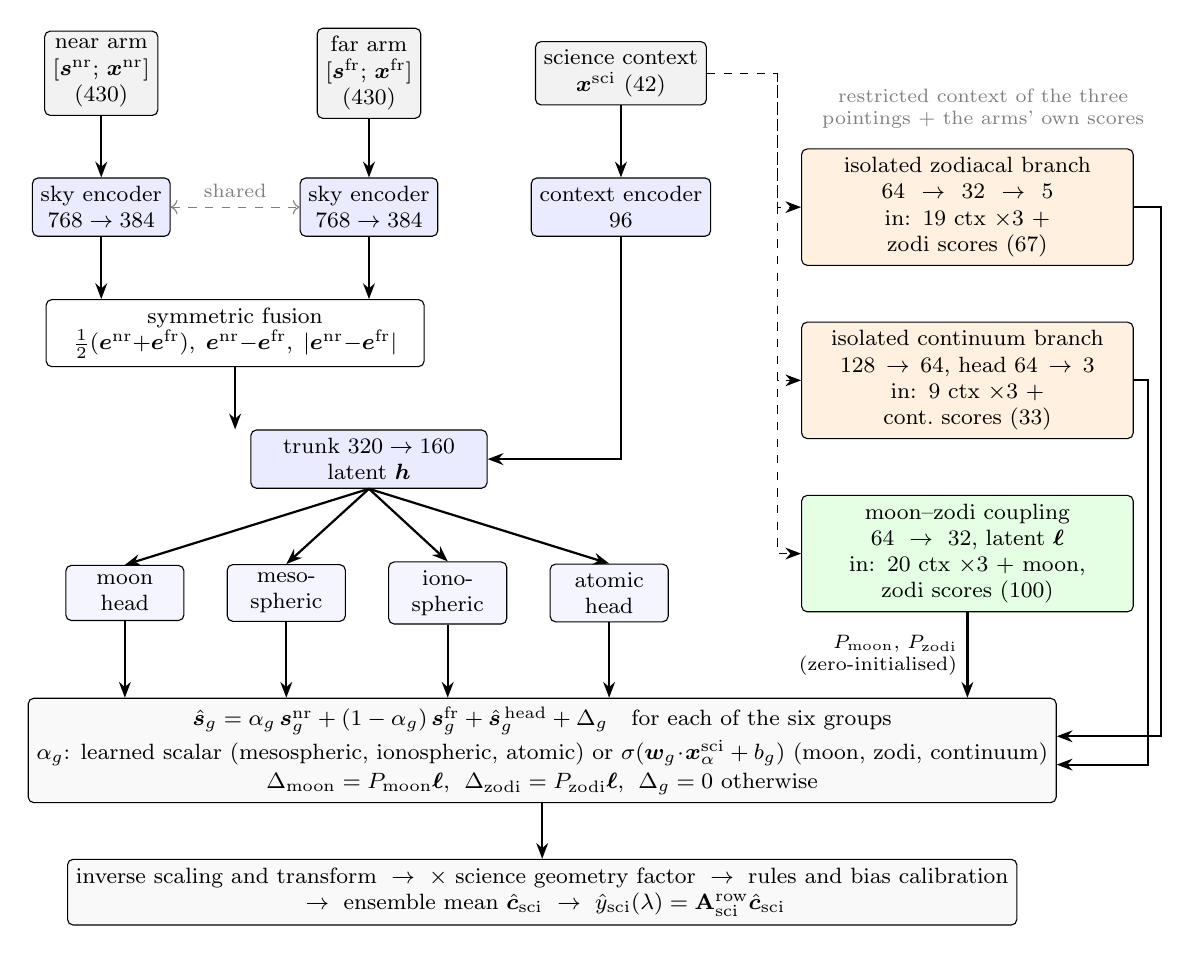
\begin{tikzpicture}[
  font=\footnotesize,
  box/.style={draw, rounded corners=2pt, align=center, minimum height=7mm,
              inner sep=3pt, fill=white},
  xinp/.style={box, fill=gray!10},
  xenc/.style={box, fill=blue!8},
  xiso/.style={box, fill=orange!12},
  xcpl/.style={box, fill=green!10},
  xhead/.style={box, fill=blue!4, minimum width=15mm},
  xout/.style={box, fill=gray!5},
  arr/.style={-{Stealth[length=2mm]}, thick},
  darr/.style={-{Stealth[length=2mm]}, dashed},
  node distance=6mm and 5mm]

% inputs
\node[xinp] (inN) at (0,0) {near arm\\$[\vect s^{\rm nr};\,\vect x^{\rm nr}]$\\(430)};
\node[xinp] (inF) at (3.4,0) {far arm\\$[\vect s^{\rm fr};\,\vect x^{\rm fr}]$\\(430)};
\node[xinp] (inS) at (6.6,0) {science context\\$\vect x^{\rm sci}$ (42)};

% encoders
\node[xenc] (encN) at (0,-1.7) {sky encoder\\$768\to384$};
\node[xenc] (encF) at (3.4,-1.7) {sky encoder\\$768\to384$};
\node[xenc] (encC) at (6.6,-1.7) {context encoder\\$96$};
\draw[<->, dashed, gray] (encN.east) -- node[above, font=\scriptsize, text=gray]{shared} (encF.west);

% fusion
\node[box, minimum width=48mm] (fus) at (1.7,-3.3)
  {symmetric fusion\\$\tfrac12(\vect e^{\rm nr}{+}\vect e^{\rm fr}),\;
   \vect e^{\rm nr}{-}\vect e^{\rm fr},\;|\vect e^{\rm nr}{-}\vect e^{\rm fr}|$};

% trunk
\node[xenc, minimum width=30mm] (trunk) at (3.4,-4.9) {trunk $320\to160$\\latent $\vect h$};

% heads
\node[xhead] (hM) at (0.3,-6.6) {moon\\head};
\node[xhead] (hO) at (2.35,-6.6) {meso-\\spheric};
\node[xhead] (hI) at (4.4,-6.6) {iono-\\spheric};
\node[xhead] (hA) at (6.45,-6.6) {atomic\\head};

% isolated branches and coupling (right column)
\node[xiso, text width=40mm] (zb) at (11.0,-1.7)
  {isolated zodiacal branch\\$64\to32\to5$\\in: 19 ctx $\times3$ + zodi scores (67)};
\node[xiso, text width=40mm] (cb) at (11.0,-3.9)
  {isolated continuum branch\\$128\to64$, head $64\to3$\\in: 9 ctx $\times3$ + cont.\ scores (33)};
\node[xcpl, text width=40mm] (mz) at (11.0,-6.1)
  {moon--zodi coupling\\$64\to32$, latent $\vect\ell$\\in: 20 ctx $\times3$ + moon, zodi scores (100)};

% arrows main path
\draw[arr] (inN) -- (encN);
\draw[arr] (inF) -- (encF);
\draw[arr] (inS) -- (encC);
\draw[arr] (encN) -- (encN|-fus.north);
\draw[arr] (encF) -- (encF|-fus.north);
\draw[arr] (fus.south) -- (fus.south|-trunk.north);
\draw[arr] (encC.south) |- (trunk.east);
\foreach \h in {hM,hO,hI,hA} \draw[arr] (trunk.south) -- (\h.north);

% inputs to side branches
\draw[darr] (inS.east) -- ++(0.9,0) |- (zb.west);
\draw[darr] (inS.east) ++(0.9,0) |- (cb.west);
\draw[darr] (inS.east) ++(0.9,0) |- (mz.west);
\node[font=\scriptsize, align=center, text=gray] at (11.2,-0.45)
  {restricted context of the three\\pointings + the arms' own scores};

% blend / output row
\node[xout, minimum width=128mm] (blend) at (5.6,-8.6)
  {$\hat{\vect s}_g = \alpha_g\,\vect s^{\rm nr}_g + (1-\alpha_g)\,\vect s^{\rm fr}_g
   + \hat{\vect s}^{\,\rm head}_g + \Delta_g$\quad for each of the six groups\\[1pt]
   $\alpha_g$: learned scalar (mesospheric, ionospheric, atomic) or
   $\sigma(\vect w_g\!\cdot\!\vect x^{\rm sci}_\alpha + b_g)$ (moon, zodi, continuum)\\[1pt]
   $\Delta_{\rm moon}=P_{\rm moon}\vect\ell$, \;$\Delta_{\rm zodi}=P_{\rm zodi}\vect\ell$,
   \;$\Delta_g = 0$ otherwise};

\foreach \h in {hM,hO,hI,hA} \draw[arr] (\h.south) -- (\h.south|-blend.north);
\draw[arr] (zb.east) -- ++(0.35,0) |- ($(blend.east)+(0,0.18)$);
\draw[arr] (cb.east) -- ++(0.18,0) |- ($(blend.east)+(0,-0.18)$);
\draw[arr] (mz.south) -- node[left, font=\scriptsize, align=right]
  {$P_{\rm moon}$, $P_{\rm zodi}$\\(zero-initialised)} (mz.south|-blend.north);

% final
\node[xout] (final) at (5.6,-10.4)
  {inverse scaling and transform $\;\to\;$ $\times$ science geometry factor
   $\;\to\;$ rules and bias calibration\\
   $\;\to\;$ ensemble mean $\hat{\vect c}_{\rm sci}$
   $\;\to\;$ $\hat y_{\rm sci}(\lambda) = \mathbf{A}^{\rm row}_{\rm sci}\hat{\vect c}_{\rm sci}$};
\draw[arr] (blend) -- (final);
\end{tikzpicture}
\caption{Architecture of the transfer network. Grey: inputs; blue: shared
encoders, trunk and trunk-fed heads; orange: isolated branches for the
zodiacal and diffuse-continuum groups; green: the additive moon--zodiacal
coupling. Numbers give layer widths and input dimensions. The last row lists
the post-processing of Sections~\ref{sec:compression}, \ref{sec:normalisation},
\ref{sec:rules} and \ref{sec:calibration}.}
\label{fig:arch}
\end{figure*}

\paragraph{Context routing.} Every context feature enters both arm encoders
and the context encoder, and hence the trunk. The isolated branches, the
coupling branch and the blend predictor see only the restricted sets of
Table~\ref{tab:routing}; Table~\ref{tab:heads} lists which upstream path
feeds each head. A feature absent from a restricted set never reaches the
corresponding head. The two anchor inputs therefore had to be added to the
zodiacal set explicitly: without them the zodiacal head would be asked to
reproduce a ceiling defined by a prediction it could not see.

\begin{deluxetable}{lcccc}
\tablecaption{Context features read by the restricted
paths.\label{tab:routing}}
\tablehead{\colhead{Feature} & \colhead{Zodi} & \colhead{Continuum} &
  \colhead{Coupling} & \colhead{$\alpha_g$}}
\startdata
Pointing altitude & \yes & & & \\
Pointing azimuth ($\sin$, $\cos$) & & & & \\
Airmass & \yes & \yes & \yes & \yes \\
Moon altitude, Moon separation & \yes & \yes & \yes & \\
Lunar phase ($\sin$, $\cos$) & \yes & \yes & \yes & \\
Moon azimuth ($\sin$, $\cos$) & & & & \\
Solar elongation & \yes & & \yes & \\
Sun altitude & \yes & & & \\
Sun azimuth ($\sin$, $\cos$) & & & & \\
Separation from science pointing, telescope identity & & & & \\
Van Rhijn factor, 87 and 95\,km & & & & \\
Van Rhijn factor, 285\,km & \yes & & \yes & \\
Time of night, lunation, year & & & & \\
Solar and geomagnetic activity & & & & \\
Ecliptic latitude & \yes & & \yes & \yes \\
Ecliptic longitude ($\sin$, $\cos$) & \yes & & \yes & \\
Tabulated zodiacal brightness & \yes & & \yes & \\
FLI & \yes & \yes & \yes & \\
Horizon step $u$ & \yes & & \yes & \yes \\
Lunar airmass, moonlight proxy $S$ & \yes & & \yes & \\
${\rm FLI}\cos\phi$ & & \yes & \yes & \\
$S\cos\lambda_{\rm ecl}$, $S\sin\lambda_{\rm ecl}$ & & \yes & \yes & \\
Predicted moonlight ratio & & & & \\
$\log_{10}Z_{\rm pred}$, $f_{\rm pred}$ & \yes & & \yes & \\
\hline
Number of features & 19 & 9 & 20 & 3 \\
\enddata
\tablecomments{Columns: isolated zodiacal branch, isolated continuum branch,
moon--zodiacal coupling branch, and the context-dependent blend weight
$\alpha_g$. All features also reach the shared trunk.}
\end{deluxetable}

\begin{deluxetable}{lcccc}
\tablecaption{Upstream path feeding each group head.\label{tab:heads}}
\tablehead{\colhead{Head} & \colhead{Shared trunk} & \colhead{Isolated zodi} &
  \colhead{Isolated continuum} & \colhead{Coupling (additive)}}
\startdata
Moon        & \yes & & & \yes \\
Zodi        & & \yes & & \yes \\
Continuum   & & & \yes & \\
Mesospheric & \yes & & & \\
Ionospheric & \yes & & & \\
Atomic      & \yes & & & \\
\enddata
\end{deluxetable}

\subsection{Arm-blend prior}
\label{sec:blend}

A good first estimate of the science coefficients is an interpolation between
the two sky arms. The blend term of Equation~(\ref{eq:output}) makes that estimate
explicit, and the heads predict a residual on top of it.
\begin{itemize}
  \item \emph{Isotropic groups.} For the mesospheric, ionospheric and atomic
        groups, whose transfer is isotropic on the LVM baseline, $\alpha_g$
        is a learned scalar clipped to $[10^{-3}, 1-10^{-3}]$.
  \item \emph{Anisotropic groups.} For the moon, zodiacal and continuum
        groups it depends on the science context,
        \begin{equation}
          \alpha_g(\vect x^{\rm sci}) = \sigma\big(\vect w_g\cdot\vect x^{\rm sci}_\alpha + b_g\big),
        \end{equation}
        where $\vect x^{\rm sci}_\alpha$ contains the horizon step, the
        ecliptic latitude and the airmass. The weights $\vect w_g$ are
        initialised to zero and $b_g$ to the logit of the initial blend, so
        training starts from a context-independent blend. Extending the
        context-dependent blend to all six groups degrades the ionospheric
        group.
  \item \emph{Learning rate.} The loss is nearly flat in $\alpha$: the head
        absorbs the systematic part of a mis-set blend, but not the per-row
        arm noise that the blend passes through. A wrong $\alpha$ therefore
        costs accuracy while generating little gradient, and the sigmoid
        damps it further. The blend parameters are therefore trained with a
        learning rate 30 times that of the rest of the network. With this,
        $\alpha$ reaches the same optimum from either side of the
        initialisation instead of remaining where it started.
  \item \emph{Learned values.} The blend weights favour the near arm for
        every group, between about 0.79 (mesospheric) and 0.95
        (ionospheric). Directly copying the near arm is also a better naive
        predictor than the arm mean for all six groups. The zodiacal blend
        sits near 0.9 rather than the 0.5 an isotropic emitter would
        suggest, consistent with the zodiacal family also carrying continuum
        that is not zodiacal light.
\end{itemize}
The blend predictor reads only the science context. It can learn regime
dependence, but not which arm is better placed, which would require the
difference between the arms' contexts.

\subsection{Loss}
\label{sec:loss}

The loss mixes flux space and score space. The moon, zodiacal and continuum
groups, whose errors matter in proportion to their brightness, are compared
as reconstructed spectra. The line groups are compared in score space, where
the robust scaling makes residuals comparable across coefficients of very
different amplitude.

\paragraph{Flux-space term.} For $g\in\{\text{moon, zodi, continuum}\}$ the
predicted and target scores are passed through a differentiable
implementation of the inverse transform:
\begin{enumerate}
  \item robust scaling;
  \item rotation;
  \item standardisation;
  \item elementwise square;
  \item multiplication by the science-pointing geometry factor.
\end{enumerate}
Both are then projected onto the continuum templates $\mathbf{T}_g$ of the
sample's own basis, on the full native wavelength grid. The per-row term is
\begin{equation}
  \mathcal{L}^{\rm flux}_{g,r} = s_g\,\frac{1}{n_\lambda}\sum_{\lambda}
  w_{r\lambda}\,\big[(\hat{\vect c}_{g,r}-\vect c_{g,r})^{\!\top}\mathbf{T}_g\big]_\lambda^2 ,
\end{equation}
The terms are:
\begin{itemize}
  \item $w_{r\lambda} = 1/(y_{r\lambda}\,s(\lambda))$ is the photon-noise
        weight of the total observed science flux, with a variance floor of
        5\% of the row median, normalised to unit mean per row;
  \item $s_g$ matches the median per-row flux term to the median per-row
        score-space term, so the group weights below keep their meaning.
\end{itemize}
Unlike a score-space loss with inverse-variance weights, this term couples
the weight of a row to the brightness of its target. A given score error on a
bright-Moon row, where the sky subtraction is most at risk, costs up to
$10^5$ times more than on a dark row, matching its effect on the delivered
spectrum. Each group is compared through its own templates only; no sum of
groups is constrained.

\paragraph{Log-amplitude term.} The flux term is absolute and is dominated by
the brightest rows. For the moon group, a scale-free companion penalises
fractional amplitude errors equally at all brightnesses:
\begin{equation}
  \mathcal{L}^{\rm amp}_{{\rm moon},r} = \lambda_{\rm amp}\left[\log\frac{\sum_\lambda\hat f_r(\lambda)+\epsilon}{\sum_\lambda f_r(\lambda)+\epsilon}\right]^2,
  \qquad \lambda_{\rm amp} = 5,
\end{equation}
Here $f$ is the moon flux and $\epsilon$ is 5\% of its median training
amplitude, so rows far below typical brightness do not dominate the ratio.
The zodiacal group has no such term. Its amplitude is set by the anchor on
most moon-up rows, so an additional amplitude penalty would only trade
spectral shape for an amplitude the network already reproduces.

\paragraph{Score-space term.} For the mesospheric, ionospheric and atomic
groups,
\begin{equation}
  \mathcal{L}^{\rm score}_{g,r} = \frac{1}{n_g}\sum_{k=1}^{n_g} w^{\rm pe}_{g,k,r}\;
  \mathrm{Huber}\big(\hat s_{g,k,r}-s_{g,k,r}\big),
\end{equation}
Here $\mathrm{Huber}$ is quadratic for residuals below one (in scaled units)
and linear beyond. The per-element weights $w^{\rm pe} = 1/\sigma_s^2$
propagate the decomposition uncertainties (Section~\ref{sec:uncertainties})
through the transform to first order,
$\sigma_{s,k} = \lVert\nabla_{\vect c_g} s_k\rVert\,\sigma_{\vect c_g}$,
divided by the robust score scale. Two further details:
\begin{itemize}
  \item $\sigma_s$ has a floor at 5\% (20\% for the mesospheric and atomic
        groups, whose uncertainty distributions have tails spanning three to
        six decades) of the per-coefficient median;
  \item the weights are normalised to unit mean over the training rows.
\end{itemize}

\paragraph{Total.} The total loss is
\begin{equation}
  \mathcal{L} = \frac{1}{6}\sum_g \frac{m_g}{\sqrt{n_g}}\;
  \Big\langle \mathcal{L}_{g,r}\Big\rangle_r ,
\end{equation}
with group weights $m_{\rm moon} = 3$, $m_{\rm zodi} = 2$ and $m_g = 1$
otherwise, and $\mathcal{L}_{g,r}$ the flux (plus amplitude) term or the score term as
appropriate. Rows are weighted uniformly: per-regime reweighting was tested
and did not help.

\subsection{Constraint-derived amplitudes}
\label{sec:rules}

In each half of the sample one continuum amplitude is fixed by a constraint
of the decomposition rather than by the data (Table~\ref{tab:occupancy}).
There the target is a known function of geometry, so it is derived at
prediction time instead of learned. Both rules have three properties:
\begin{itemize}
  \item they rescale a whole coefficient block and leave the predicted
        spectral shape unchanged;
  \item they are idempotent;
  \item they are linear in the coefficients, so the ensemble mean of
        members that satisfy them satisfies them too.
\end{itemize}
The zodiacal rule is applied first, because the moonlight rule reads the
predicted zodiacal amplitude.

\paragraph{Bright Moon: the zodiacal ceiling.} Where the anchor binds, the
zodiacal integral equals $\kappa_z C Z_{\rm pred}$ exactly. With $S$ fitted
on the training rows, the rule acts in two ways:
\begin{itemize}
  \item it clips the predicted zodiacal amplitude to $S Z_{\rm pred}$ on
        every row. This is a hard upper bound on the fitted value, exceeded
        on 0.01\% of rows and never by more than 0.002\,dex, so clipping can
        only move a prediction toward the truth;
  \item on rows with $f_{\rm pred} > 0.6$ it sets the amplitude to the
        ceiling when the network already predicts at least 90\% of it.
\end{itemize}
The second condition preserves genuinely interior rows, which the network
places well below the ceiling. The loss is left unchanged on these rows. The
network learns the ceiling, and its own prediction is what separates pinned
from interior rows.

\paragraph{Dark time: the moonlight floor.} Where the moon-share bracket has
collapsed onto its floor, the moonlight is not measured (Section~\ref{sec:constraints}):
\begin{itemize}
  \item \emph{Training.} The flux loss is made amplitude-blind on these rows:
        the prediction is rescaled to the true integral before the flux term
        (with the scale factor kept in the gradient, so that the amplitude
        gradient vanishes identically), and the log-amplitude term is
        dropped. Only the shape is trained.
  \item \emph{Prediction.} The amplitude is restored from the near arm's
        measured moonlight-to-zodiacal ratio,
        \begin{equation}
        \begin{split}
          \textstyle\int{\rm moon}_{\rm sci} = {}&\mathrm{clip}\big(
          (\textstyle\int{\rm moon}/\!\int{\rm zodi})_{\rm nr},\,0,\,R\big)\\
          &\times\textstyle\int{\rm zodi}_{\rm sci},
        \end{split}
        \end{equation}
        with the fitted constant $R\approx\epsilon/(1-\epsilon)$ as a
        fallback when the near arm is unusable. The ratio is transferred,
        rather than set to $R$, because the moon share of dark rows is
        bimodal: 96\% of such rows sit on the floor and about 3\% want no
        moonlight at all.
  \item \emph{Gate.} The regime is selected by
        $f_{\rm pred}\le\epsilon/\kappa_f$, not by lunar altitude. Scattered
        moonlight with the Moon a few degrees below the horizon is real, and
        the horizon taper multiplies phase and separation: a thin crescent
        $2^\circ$ down contributes nothing, while a full Moon $5^\circ$ down
        still does. No fixed altitude cut matches the predicted-fraction
        gate in both coverage and exactness (Table~\ref{tab:moongate}).
\end{itemize}

\begin{deluxetable}{lccc}
\tablecaption{Dark-time gate.\label{tab:moongate}}
\tablehead{\colhead{Gate} & \colhead{Coverage} & \colhead{Pinned} &
  \colhead{$|\Delta|>0.05$\,dex}}
\startdata
$h_{\rm moon}\le0^\circ$ & 49.7\% & 92.6\% & 7.4\% \\
$h_{\rm moon}\le-4^\circ$ & 47.0\% & 96.1\% & 3.9\% \\
$h_{\rm moon}\le-12^\circ$ & 41.4\% & 95.7\% & 4.2\% \\
$f_{\rm pred}\le\epsilon/\kappa_f = 0.0067$ & 47.8\% & 96.2\% & 3.7\% \\
\enddata
\tablecomments{Fraction of rows covered, fraction of covered rows actually
pinned at the moon-share floor, and fraction whose amplitude differs from the
floor by more than 0.05\,dex.}
\end{deluxetable}

\paragraph{Degenerate continuum.} The dark rows that want no moonlight are
failed fits rather than a physical state. Their median reduced $\chi^2$ is 15
times that of healthy dark rows, and all of their continuum is in the
zodiacal family. They are flagged at prediction time using only the two sky
arms: both arms have a moonlight-to-zodiacal ratio below $R/2$. This flag has
88\% precision at 95\% recall, affects 1.9\% of rows, and never fires with
the Moon up.

\subsection{Bias calibration}
\label{sec:calibration}

After training, a multiplicative bias correction is fitted on the training
and validation rows and applied at prediction time:
\begin{itemize}
  \item \emph{Moon and zodiacal groups.} The correction is per coefficient,
        $\ell_k = \bar c^{\rm true}_k/\bar c^{\rm pred}_k$, clipped to
        $[0.7,1.4]$. A single factor cannot remove the spectral tilt of the
        bias.
        \begin{itemize}
          \item The moon correction is fitted only on rows where the
                moonlight amplitude is predicted by the network rather than
                derived by the dark-time rule.
          \item The zodiacal correction is fitted separately in three
                lunar-altitude regimes, with smooth transitions between them.
        \end{itemize}
  \item \emph{Other groups.} A single factor per group is fitted on the
        flux-weighted amplitude $A_g = \vect c_g\cdot\vect v_g$, clipped to
        $[0.5, 2]$. For a group whose templates carry very different flux,
        the unweighted mean coefficient is a different functional from the
        flux amplitude, and the two can disagree in sign. Across the 357 OH
        templates the integrals span nine decades and are anti-correlated
        with coefficient size.
\end{itemize}

\subsection{Training}

\begin{itemize}
  \item \emph{Splits.} Rows are grouped by night and assigned to training,
        validation and test sets stratified by lunar phase. Whole nights are
        held out because the sky of neighbouring exposures within a night is
        correlated, and a random split would leak.
  \item \emph{Optimisation.} Each network is trained with AdamW
        \citep{Loshchilov2019}:
        \begin{itemize}
          \item learning rate $10^{-3}$, weight decay $2\times10^{-4}$ and
                gradient clipping at 1;
          \item batch size 512;
          \item up to 400 epochs, with early stopping on the validation loss
                and a patience of 100 epochs.
        \end{itemize}
        The blend parameters form a separate parameter group without weight
        decay and with the raised learning rate of Section~\ref{sec:blend}.
  \item \emph{Ensemble.} The prediction is the mean over an ensemble of ten
        networks trained with different random seeds on the same split. The
        ensemble spread is reported as an epistemic uncertainty.
\end{itemize}

\subsection{Evaluation}
\label{sec:evaluation}

Three considerations govern how the transfer is assessed.

\paragraph{Flux space.} The deliverable is a sky spectrum, and coefficient
errors can be misleading in flux. Coefficient-space metrics are dominated by
the 358 mesospheric coefficients, and they can disagree in sign with flux
metrics measured on the same predictions. The transfer is therefore judged
on reconstructed spectra: the photon-weighted $\chi^2$ of
$y_{\rm sci} - \hat y_{\rm sci}$, compared with the decomposition's own fit
to $y_{\rm sci}$. That comparison sets the floor below which no transfer of
decomposition coefficients can go.

\paragraph{The sky-arm floor.} A natural reference is the disagreement
between the two sky arms, $\Delta = \tfrac12\,\mathrm{rms}(\vect c^{\rm nr}-\vect c^{\rm fr})$.
If each arm carries independent noise $\sigma$, then $\Delta\approx0.71\sigma$.
A perfect predictor still scores an error $\sigma$ against a science truth
carrying its own noise, so the floor for a group whose truth is as noisy as
the arms is ${\rm err}/\Delta\approx\sqrt2$, not 1. Values well below 1 mean
that the head uses context the arms do not carry.

\paragraph{Filtered and unfiltered rows.} The selection of
Section~\ref{sec:selection} does not run in production. A change aimed at
pathological rows can appear neutral on the filtered test set because the
selection has already removed most of its targets. Conversely, a pathology
that is rare in training need not be rare in delivery. Changes are measured
on the population whose behaviour they are meant to change, and what cannot
be fixed is flagged.

\subsection{Prediction}

At prediction time the inputs are the near and far spectra of an exposure,
their decompositions, and the context of all three pointings. The steps are:
\begin{enumerate}
  \item the sky coefficients are normalised (Section~\ref{sec:normalisation})
        and transformed to scores;
  \item each ensemble member predicts the science scores
        with Equation~(\ref{eq:output});
  \item the scores are inverted to coefficients and multiplied by the
        science-pointing geometry factors;
  \item the rules of Section~\ref{sec:rules} and the calibration of
        Section~\ref{sec:calibration} are applied;
  \item the members are averaged;
  \item the science sky spectrum is reconstructed with the science
        spectrum's LSF and transmission.
\end{enumerate}
A reliability mask in the vocabulary of Table~\ref{tab:flags} accompanies
each prediction:
\begin{itemize}
  \item diffuse collapse is evaluated from the predicted coefficients;
  \item moon/zodiacal reversal is evaluated from the reconstructed continua;
  \item the degenerate-continuum flag is evaluated from the sky arms.
\end{itemize}
The constraint warnings do not apply to a prediction. They describe how the
decomposition shaped the training targets, which is a property of the sample
rather than of the prediction.

%======================================================================
\bibliography{sky_subtraction_method}{}
\bibliographystyle{aasjournalv7}

\end{document}
